\documentclass[aps,pre,twocolumn,superscriptaddress,floatfix,longbibliography]{revtex4-2}

\usepackage{amsmath,amssymb}
\usepackage{graphicx}
\usepackage[colorlinks=true,allcolors=blue]{hyperref}

\begin{document}

\title{Stark resonances under exponential-cosine screening: through-threshold
maps for the quantum-plasma hydrogen atom}

\author{C.~D.~Reinoso}
\email{cesardanielrrch@gmail.com}
\affiliation{Facultad de Ciencias, Escuela Superior Polit\'ecnica de
Chimborazo (ESPOCH), Riobamba, Ecuador}

\date{\today}

\begin{abstract}
The exponential-cosine screened Coulomb (ECSC) potential of dense
quantum plasmas differs from Debye screening in one structural
respect: its tail oscillates. We compute the resonance spectrum of
the hydrogen atom under ECSC screening combined with a static
electric field with a coupled-channel complex-scaling method,
exploiting an exact identity --- the ECSC potential is the half-sum
of two Yukawa potentials at complex screening parameters --- which
also yields the analytic rotation bound $\theta_c<\pi/4$. Three
results organize the physics. At zero field, parametric continuation
addresses the intermediate screening window left open in the
literature: within the sector that uniform complex scaling can
expose, no isolated ground pole survives beyond the critical
screening $\lambda_c=0.7205$ --- the pole merges into the rotated
continuum, consistent with the conjectured virtual-state scenario
--- while the $2p$ pole detaches at $\lambda_c(2p)=0.148205$ (all
digits confirmed by a recent 60-digit benchmark) as a genuine
resonance, rotation-stable to $10^{-13}$. With the field on, we map
the ground resonance on a $5\times19$ grid of the $(F,\lambda)$
plane: at every field strength the resonance crosses $E_r=0$ near
$\lambda^{*}\approx0.68$ --- nearly field-independent, a corollary
of the vanishing field displacement at threshold --- and continues
smoothly as a positive-energy resonance, a regime the companion
Debye map only approaches near its much larger critical screening.
Finally, comparing ECSC and Debye screening at matched binding
energy isolates the tail effect on ionization: the cosine factor
extinguishes the assisting Coulombic tail well before its first
zero, making the Stark barrier higher and wider, and suppresses the
field-ionization width by roughly a factor of two at weak field ---
a suppression that fades as the field strengthens and the barrier
peak moves inward to where the two potentials coincide.
\end{abstract}

\maketitle

\section{Introduction}

Screening in a dense, degenerate electron gas is not exponential.
Quantum hydrodynamic treatments of test-charge screening in quantum
plasmas~\cite{ShuklaEliasson2008} lead to the exponential-cosine
screened Coulomb (ECSC) potential,
\begin{equation}
V(r)=-\frac{Z}{r}\,e^{-\lambda r}\cos(\lambda r),
\label{eq:ecsc}
\end{equation}
whose study as a model interaction long predates that
derivation~\cite{LamVarshni1972}. The oscillating factor is not a
cosmetic difference from the Debye--H\"uckel form: the potential
changes sign, its tail alternates between attraction and repulsion,
and this modifies both the bound spectrum --- critical screening
parameters differ substantially~\cite{JiaoCritical2021} --- and the
resonance structure. Field-free ECSC resonances have recently been
mapped with high precision by the complex-scaling pseudospectral
work of Jiao and collaborators~\cite{JiaoHo2021}, who located the
loss of the ground state at $\lambda_c=0.720524$ and the emergence
of well-defined $s$-wave shape resonances at
$\lambda_{r+}=0.90035$, and who explicitly note that the behavior in
the intermediate window is unexplained, conjecturing conversion into
virtual states. Perturbative field responses (polarizabilities and
hyperpolarizabilities) of ECSC-screened atoms are likewise
known~\cite{PRE2023polarizabilities}, and the one nonperturbative
Stark calculation under ECSC screening --- complex-scaled resonance
energies and widths, focused on high-lying states at selected
parameter points --- was carried out by Wang, Chen, and
Guo~\cite{WangChenGuo2019}. (For Debye screening the combined
field--screening problem has a longer nonperturbative
lineage~\cite{YuHo2005,LinHo2011,companionD}.) What does not exist
for the ECSC case is systematic coverage: a resonance map of the
combined field--screening plane, the fate of excited Stark
manifolds, or a controlled comparison against Debye screening that
isolates what the oscillating tail actually does to field
ionization. This paper supplies the three.

The tool is the coupled-channel complex-scaling method of our Debye
companion study~\cite{companionD}: Eq.~(\ref{eq:ecsc}) is the
half-sum of two Yukawa potentials at complex screening parameters
$\lambda(1\pm i)$, so every screened matrix element reuses the
Debye code path at complex argument, and the identity yields at
once the analytic bound $\theta_c<\pi/4$ on the rotation angle.
The engine verifies its hydrogen limit on import --- a failed check
aborts any run --- and its Yukawa mode reproduces the companion
engine to $2\times10^{-16}$.

\section{Method}
\label{sec:method}

The $m=0$ coupled-channel complex-scaling machinery is that of
Ref.~\cite{companionD}; we restate it here so the paper is
self-contained. Each angular channel $\ell=0,\dots,\ell_{\max}$
carries the orthonormal radial functions
\begin{equation}
\varphi^{(\ell)}_i(r)=N_{i\ell}\,x^{\ell+1}e^{-x/2}
L^{(2\ell+2)}_i(x),\qquad x=2\beta r,
\end{equation}
with $L^{(a)}_i$ generalized Laguerre polynomials, $N_{i\ell}$ fixed
by $\int_0^\infty\varphi_i\varphi_j\,dr=\delta_{ij}$, and a common
scale $\beta=0.35$ for all channels; production settings are
$n_b=70$ functions per channel, $\ell_{\max}=14$ (1050 degrees of
freedom), and a shared 3000-point Gauss--Legendre quadrature on
$x\in[0,760]$ (basis-overlap identity certified to
$1.3\times10^{-12}$ on every constructed basis, so the problem is a
standard complex-symmetric eigenproblem). Adjacent channels couple
through the dipole blocks
$(\ell+1)/\sqrt{(2\ell+1)(2\ell+3)}\,\langle\varphi_i|r|
\varphi_j\rangle$, and every operator is scaled
analytically~\cite{AguilarCombes1971,BalslevCombes1971,Ho1983,
Reinhardt1982,Moiseyev1998}; the Stark term is covered by the
Herbst--Simon theory~\cite{HerbstSimon1978,Herbst1979}. The single
ECSC-specific element is the screened factor: writing $e^{-\lambda
r}\cos\lambda r=\tfrac12[e^{-\mu_+r}+e^{-\mu_-r}]$ with
$\mu_\pm=\lambda(1\pm i)$, the complex-scaled screening enters as
two Yukawa evaluations at $\mu_\pm re^{i\theta_c}$. Decay of these
factors requires $\mathrm{Re}(\mu_\pm e^{i\theta_c})>0$, i.e.
\begin{equation}
\theta_c<\pi/4,
\end{equation}
a hard analytic cap (enforced in the code) comfortably above the
production angles $\theta_c=0.18/0.28$ (retry $0.30/0.42$).
Resonances are identified by parametric continuation: at each new
$\lambda$ the search window is centered on
$E_{\mathrm{pred}}=E_b^{F=0}(\lambda)+[E(\lambda_{\mathrm{prev}})
-E_b^{F=0}(\lambda_{\mathrm{prev}})]$ while the bound level exists,
and on complex linear extrapolation beyond; the eigenvalue nearest
the prediction at $\theta_c=0.18$ is paired with the eigenvalue
nearest \emph{it} at $0.28$, and the pair is accepted if the
modulus difference --- recorded as the spread --- is below a
width-scaled tolerance. ($\theta_c$-trajectories over
$[0.14,0.50]$ are computed for the least favorable points.)
Uncertainties quoted are these spreads --- error estimates
calibrated against the anchors below, not bounds.

Verification. The hydrogen limit reproduces $-1/2n^{2}$ to
$7\times10^{-11}$ --- the check runs at engine import and a failure
raises, so no production run can proceed on a failed assembly; the
$\lambda=0$ row of the production map reproduces the pure-Stark
anchors of Ref.~\cite{companionD} (themselves validated to ten
digits against the classical Stark values~\cite{DamburgKolosov1976,
Kolosov1987,Jentschura2001}); the small-$\lambda$ expansion of the
ground level follows the exact law $E_{1s}=-\tfrac12+\lambda
-\lambda^{3}\langle r^{2}\rangle/3+O(\lambda^{4})$ --- the
$\lambda^{2}$ term is absent for ECSC, unlike Debye screening ---
to the expected order (deviation $1.2\times10^{-8}$ at
$\lambda=0.01$). For the critical screenings, a 60-digit benchmark
has recently become available~\cite{Bunker2026}: our
$\lambda_c(2p)=0.148205$ agrees with its
$0.148205032\ldots$ on all quoted digits, and our variational
$\lambda_c(1s)=0.72027$ sits within the documented
threshold-diffusivity bias~\cite{companionNR} of the exact
$0.720524085\ldots$~\cite{Bunker2026,JiaoCritical2021}. The tables
of Ref.~\cite{WangChenGuo2019} concern high-lying resonances and
contain no ground-state data overlapping the present map; a
comparison at their excited-state points is planned once their
tabulation is at hand.

\section{Results}
\label{sec:results}

\subsection{Field-free pole structure: the intermediate window}
\label{sec:fieldfree}

Reference~\cite{JiaoHo2021} leaves open what happens between
$\lambda_c=0.720524$, where the ground state ceases to be bound, and
$\lambda_{r+}=0.90035$, where sharp $s$-wave shape resonances
appear. Parametric continuation addresses this within a precisely
stated scope. Tracking the $1s$ pole across $\lambda_c$ with fine
steps, the pole moves smoothly and basis-stably into the lower half
plane, but its rotation response degrades monotonically: the
two-angle spread grows from $5\times10^{-5}$ at $\lambda=0.715$ to
$10^{-2}$ at $\lambda=1.25$, no $\theta_c$-plateau develops, and
--- the decisive diagnostic --- the tracked ratio $(\Gamma/2)/E_r$
converges to $\tan2\theta_c$ of the rotation angle used, the
textbook signature of the discretized rotated-continuum
ray~\cite{Reinhardt1982,Ho1983,Moiseyev1998} rather than of an
isolated pole. The statement this establishes is a null result
\emph{within uniform complex scaling}, which can only expose poles
with $(\Gamma/2)/E_r<\tan2\theta_{\max}\approx1.1$ at the ECSC cap:
in that sector, no isolated $1s$ resonance survives in the
intermediate window --- the pole merges into the continuum. A true
second-sheet virtual state is invisible to the method by
construction, so the result is consistent with --- though not a
proof of --- the virtual-state scenario conjectured in
Ref.~\cite{JiaoHo2021}; a definitive second-sheet statement would
require exterior scaling or Jost-function continuation. (The sharp
tail resonances above $\lambda_{r+}$ live too close to the rotated
ray for the present uniform-scaling setup; we do not attempt to
reproduce them and refer to Ref.~\cite{JiaoHo2021}.) The
ray-versus-pole criterion itself is standard~\cite{Reinhardt1982,
Ho1983,Moiseyev1998}; what we found operationally decisive near
threshold is applying it in ratio form together with
$\lambda$-insensitivity: any candidate whose width-to-position
ratio tracks $\tan2\theta_c$, or whose parameters do not move with
$\lambda$, is a discretized ray state, not a resonance.

The $\ell=1$ story is the clean counterpart
(Fig.~\ref{fig:2p}). The $2p$ level unbinds at
$\lambda_c(2p)=0.148205$ --- earlier than the Debye value
$0.220217$~\cite{companionNR,JiaoCritical2021}, the oscillating
tail screens harder at distance --- and detaches as a genuine shape
resonance behind the centrifugal-plus-tail barrier: near threshold
the two-angle spread is at machine level ($10^{-13}$), and the
resonance broadens rapidly as $\lambda$ grows, reaching
$\Gamma\sim\!5\times10^{-2}$ by $\lambda=0.24$.

\begin{figure}[tb]
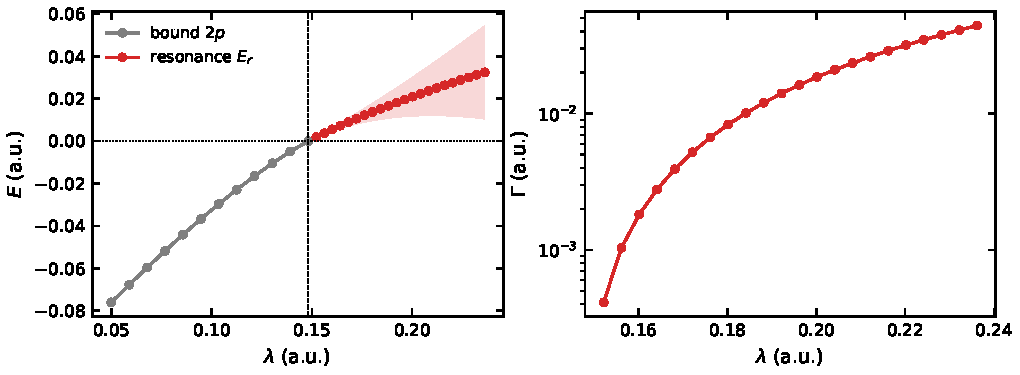
\includegraphics[width=\columnwidth]{figures/figE_2p}
\caption{\label{fig:2p}Field-free $2p$ pole under ECSC screening:
bound branch (gray), and the shape resonance born at
$\lambda_c(2p)=0.148205$ (red; band $=\pm\Gamma/2$). Right: width
on a log scale.}
\end{figure}

\subsection{The ground-state $(F,\lambda)$ map: through the
threshold}

Figure~\ref{fig:map} shows the ground-state resonance on the grid
$F\in\{0.02,\dots,0.10\}\times\lambda\in\{0,0.05,\dots,0.90\}$: all
$95$ points tracked by continuation with zero losses, two-angle
spreads below $1.5\times10^{-4}$ at the broadest corner and below
$10^{-7}$ over $58\%$ of the grid (machine-readable tables
provided).
Table~\ref{tab:map} lists a subset.

\begin{figure*}[tb]
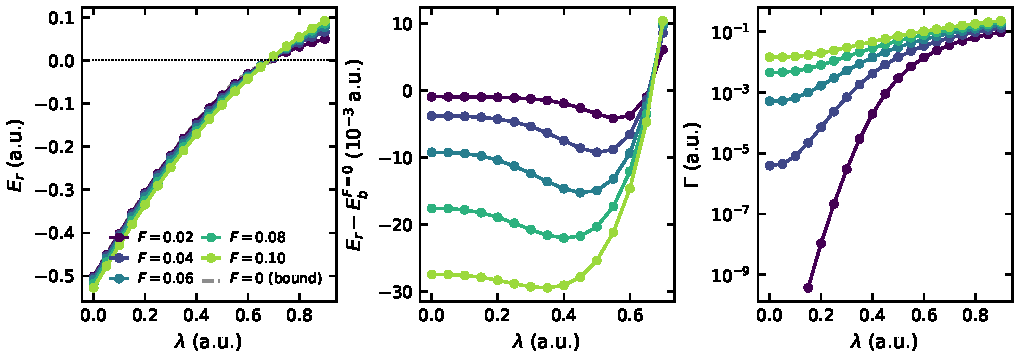
\includegraphics[width=\textwidth]{figures/figE_map}
\caption{\label{fig:map}Ground-state resonance across the
$(F,\lambda)$ plane under ECSC screening. Left: position $E_r$
(dashed: $F=0$ bound level; dotted: $E_r=0$). Center: field-induced
displacement relative to the bound level (plotted where the $F=0$
level exists). Right: width (log scale; points shown where $\Gamma$
exceeds ten times the spread).}
\end{figure*}

\begin{table}[tb]
\caption{\label{tab:map}Ground-state resonance parameters (a.u.)
at selected screenings. Widths marked $<10^{-10}$ are below the
resolved level. $\lambda^{*}$ is the $E_r=0$ crossing (linear
interpolation, $\pm0.01$). Maximum two-angle spread on the full
grid: $1.3\times10^{-4}$.}
\begin{ruledtabular}
\begin{tabular}{clccc}
$F$ & $\lambda$ & $E_r$ & $\Gamma$ & $\lambda^{*}$ \\
\hline
0.02 & 0.3 & $-0.220638$ & $3.00\times10^{-6}$ & 0.686 \\
     & 0.6 & $-0.032042$ & $1.43\times10^{-2}$ & \\
     & 0.9 & $+0.049297$ & $9.66\times10^{-2}$ & \\
0.04 & 0.3 & $-0.224766$ & $7.00\times10^{-4}$ & 0.681 \\
     & 0.6 & $-0.034837$ & $3.43\times10^{-2}$ & \\
     & 0.9 & $+0.066174$ & $1.35\times10^{-1}$ & \\
0.06 & 0.3 & $-0.231777$ & $5.27\times10^{-3}$ & 0.681 \\
     & 0.6 & $-0.037618$ & $5.62\times10^{-2}$ & \\
     & 0.9 & $+0.076982$ & $1.68\times10^{-1}$ & \\
0.08 & 0.3 & $-0.240144$ & $1.54\times10^{-2}$ & 0.681 \\
     & 0.6 & $-0.040327$ & $7.95\times10^{-2}$ & \\
     & 0.9 & $+0.085034$ & $1.99\times10^{-1}$ & \\
0.10 & 0.3 & $-0.248664$ & $3.04\times10^{-2}$ & 0.682 \\
     & 0.6 & $-0.042906$ & $1.04\times10^{-1}$ & \\
     & 0.9 & $+0.091514$ & $2.30\times10^{-1}$ & \\
\end{tabular}
\end{ruledtabular}
\end{table}

The headline is the left panel: at every field strength the ground
resonance crosses $E_r=0$ at $\lambda^{*}\approx0.68$ (from $0.686$
at $F=0.02$ to $0.681$--$0.682$ at stronger fields, a shallow
minimum near $F=0.06$; total variation below $0.01$) and continues
smoothly to positive energies, reaching $E_r=+0.049$,
$\Gamma=0.097$ at $F=0.02$, $\lambda=0.9$. The near
field-independence of $\lambda^{*}$ is a corollary of the center
panel: the field-induced displacement collapses toward zero as
$\lambda\to\lambda^{*}$ for every $F$, so the crossing location is
pinned by the screening alone. The contrast with the field-free
limit is structural: for $F\neq0$ the complex-scaled Stark operator
has empty essential spectrum~\cite{Herbst1979,HerbstSimon1978} ---
there is no continuum ray at threshold to absorb the pole, every
eigenvalue is a discrete resonance, and the crossing is guaranteed
smooth --- whereas at $F=0$ the same pole merges into the rotated
continuum within our method's resolution
(Sec.~\ref{sec:fieldfree}). A probe of the connection between the
two regimes at the $\lambda=0.90$--$0.95$ edge makes this concrete:
tracking the resonance down in field, it remains cleanly isolated
(spreads $10^{-7}$--$4\times10^{-9}$) to $F\approx0.003$, with
$(\Gamma/2)/E_r$ climbing from $0.98$ toward the exposure boundary
$\tan2\theta_{\max}\approx1.1$, below which tracking degrades ---
the pole exits the sector uniform scaling can expose as the field
is removed, consistently with the field-free merging and with no
sign, along this path, of connecting to a narrow tail resonance.
On the Debye side, the companion map~\cite{companionD} never
reaches such a crossing --- but that comparison is at equal
$\lambda$, which Sec.~\ref{sec:matched} argues is not the right
variable: in units of the respective critical screenings the ECSC
crossing sits at $\lambda^{*}/\lambda_c\approx0.94$, while the
Debye analog would require $\lambda\approx\lambda_c=1.19$, far
beyond the mapped range. The physical statement is that the ECSC
scale compression brings the positive-energy--ground regime ---
tabulated for Debye screening only at extreme
parameters~\cite{YuHo2005} --- down into the moderate-screening
window.

Two secondary features mirror the Debye map~\cite{companionD} and
one does not. Screening again catalyzes field ionization (right
panel: at $F=0.02$ the width climbs eight orders of magnitude
across the grid), and the perturbative Stark regime again shrinks
with screening. The non-mirroring feature is the field
displacement (center panel): it turns \emph{positive} as
$\lambda\to\lambda_c$, i.e.\ near the critical screening the field
\emph{raises} the resonance position relative to the vanishing
bound level --- a threshold effect absent from the Debye map at
comparable screenings.

\subsection{Debye versus ECSC at matched binding: what the
oscillating tail does to ionization}
\label{sec:matched}

The comparison that isolates the tail effect must remove the
trivial difference --- at equal $\lambda$ the two potentials bind
differently. We therefore match the \emph{binding}: for each anchor
$E_b$ we solve for $\lambda_{\mathrm{Y}}$ (Yukawa) and
$\lambda_{\mathrm{E}}$ (ECSC) such that the field-free ground level
equals $E_b$ to $10^{-9}$, then compare the Stark widths at equal
$F$. Table~\ref{tab:matched} shows the result: at matched binding
the ECSC width is systematically \emph{smaller} --- by about a
factor of two at $F=0.04$ ($\Gamma_{\mathrm{E}}/\Gamma_{\mathrm{Y}}
=0.45$--$0.57$) and less at $F=0.08$ ($0.65$--$0.82$). The
quasistatic exponent is identical by construction, so the
suppression is a pure barrier-shape effect, and its origin is the
cosine decay \emph{before} the first zero: at the $E_b=-0.30$
anchor the entire tunneling barrier lies inside
$r_0=\pi/2\lambda_{\mathrm{E}}=7.6$ (downfield barrier peak near
$r=4.4$ at $F=0.04$, outer turning point near $7.5$), and across
that region the ratio $V_{\mathrm{ECSC}}/V_{\mathrm{Y}}$ falls from
$0.89$ at $r=3$ to $0.15$ at $r=7$ --- the cosine factor
extinguishes the assisting tail well before changing its sign, so
the ECSC barrier is both higher and wider; the sign flip beyond
$r_0$ merely seals the effect. As $F$ grows the barrier peak moves
inward (to $r\approx3.3$ at $F=0.08$), into the region where the
two potentials nearly coincide, and the state approaches the
over-barrier regime --- so the suppression fades, both trends
visible in the table.

\begin{table}[tb]
\caption{\label{tab:matched}Ground Stark widths at matched
field-free binding $E_b$. $\lambda_{\mathrm{Y}},
\lambda_{\mathrm{E}}$: screening parameters at which Yukawa/ECSC
give the same $E_b$ ($10^{-9}$ match).}
\begin{ruledtabular}
\begin{tabular}{ccccc}
$E_b$ & $\lambda_{\mathrm{Y}}$ & $\lambda_{\mathrm{E}}$ & $F$ &
$\Gamma_{\mathrm{E}}/\Gamma_{\mathrm{Y}}$ \\
\hline
$-0.40$ & 0.10823 & 0.10091 & 0.04 & 0.551 \\
        &         &         & 0.08 & 0.823 \\
$-0.30$ & 0.23699 & 0.20697 & 0.04 & 0.447 \\
        &         &         & 0.08 & 0.677 \\
$-0.20$ & 0.39703 & 0.32394 & 0.04 & 0.493 \\
        &         &         & 0.08 & 0.648 \\
$-0.12$ & 0.56482 & 0.43240 & 0.04 & 0.571 \\
        &         &         & 0.08 & 0.660 \\
\end{tabular}
\end{ruledtabular}
\end{table}

\subsection{The $n=2$ doublet}

The $m=0$ doublet at $F=0.02$ (parabolic labels $k=\pm1$ assigned
by continuation from $\lambda=0$, not quantum numbers) behaves as
under Debye screening but on a compressed $\lambda$ scale,
consistent with $\lambda_c(2p)$ (Fig.~\ref{fig:manifold}): the
uphill component crosses $E_r=0$ at $\lambda\approx0.093$ (Debye:
$0.112$~\cite{companionD}) and continues to $E_r=+0.127$,
$\Gamma=0.079$ at $\lambda=0.30$; the downhill width roughly
triples over the same range ($0.061\to0.208$), with the ratio
$\Gamma_{-1}/\Gamma_{+1}$ drifting $1.97\to2.63$. Spreads are
below $10^{-5}$ except at four points (worst $6\times10^{-3}$ for
the downhill component at $\lambda=0.30$, which we quote to two
digits only).

\begin{figure}[tb]
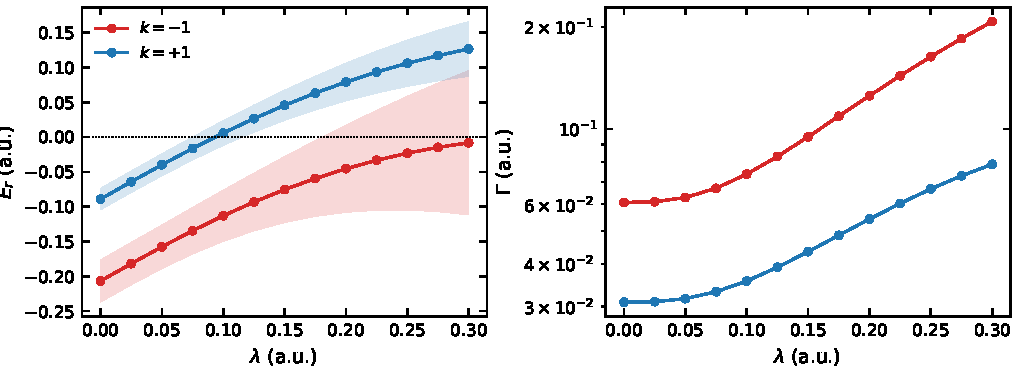
\includegraphics[width=\columnwidth]{figures/figE_manifold}
\caption{\label{fig:manifold}The $n=2$, $m=0$ Stark doublet at
$F=0.02$ under ECSC screening. Left: positions with $\pm\Gamma/2$
bands; $k$ labels the $\lambda=0$ parabolic character, carried by
continuation. Right: widths.}
\end{figure}

\subsection{Physical scope}

In the quantum-hydrodynamic derivation~\cite{ShuklaEliasson2008}
$\lambda$ is the quantum screening wavenumber, so
$\lambda=0.1$--$0.9$~a.u.\ corresponds to screening lengths of
$1$--$10\,a_0$ ($0.05$--$0.5$~nm) --- metallic to
warm-dense-matter electron densities, roughly
$10^{22}$--$10^{24}\;\mathrm{cm}^{-3}$. The ECSC form is itself a
model whose validity at the extremes remains under
discussion~\cite{PRE2023polarizabilities}; the present map is a
statement about that model's spectral content, in the same spirit
as the Debye-model literature it extends, and the matched-binding
comparison of Sec.~\ref{sec:matched} is designed to be the
model-robust part of the physics: it isolates a barrier-shape
mechanism (tail extinction before the first zero) that any
oscillatory screening form shares qualitatively.

\section{Conclusions}

Three results: the intermediate screening window of
Ref.~\cite{JiaoHo2021} is resolved --- as a null result within
uniform complex scaling, the ground pole merges into the continuum,
consistent with the virtual-state scenario; the first systematic
$(F,\lambda)$ resonance map under ECSC screening shows the ground
state crossing into a positive-energy resonance at
$\lambda^{*}\approx0.68$ for every field, pinned by the vanishing
field displacement at threshold; and the matched-binding
comparison shows the oscillating tail suppresses field ionization
by up to a factor of two, a barrier-shape effect that fades with
increasing field. The extension of the Debye machinery that made
this possible is a single identity --- the ECSC potential as a
half-sum of complex-parameter Yukawas, with its $\theta_c<\pi/4$
cap. The machinery extends unchanged to excited manifolds,
$m\neq0$, and other screening families; the relativistic (Dirac)
version of the combined problem is the natural next step and is
under way.

\begin{acknowledgments}
The author thanks the ESPOCH Faculty of Sciences for institutional
support. All scripts, gates, and machine-readable grids are
distributed with the companion programs and will be archived with a
persistent identifier at publication.
\end{acknowledgments}

\bibliography{refs}

\end{document}
